\documentclass{article}
\usepackage[utf8]{inputenc}
\usepackage{amsmath}
\usepackage{siunitx}
\usepackage{graphicx}
\usepackage{caption}
\usepackage{subcaption}
\usepackage{float}
\usepackage{enumitem}
\usepackage{amssymb}
\usepackage{pgfplots}
\usepackage[superscript]{cite}
\usepackage{todonotes}
\usepackage{tikz}
\usepackage{tabularx}
\usepackage{float}

\pgfplotsset{compat=1.16}
%\pgfplotsset{
%    dirac/.style={
%        mark=triangle*,
%        mark options={scale=1},
%        ycomb,
%        scatter,
%        visualization depends on={y/abs(y)-1 \as \sign},
%        scatter/@pre marker code/.code={\scope[rotate=90*\sign,yshift=-2pt]}
%    }
%}


\title{Implementation and Review of \\ \textit{Fast Path-Based Neural Branch Prediction\cite{fastpath}}\\ NUS CS5222, Project 1}
\author{Luca Krueger}
\date{\today}

\begin{document}
\maketitle

\section{Introduction}
This project is related to the course CS5222 Advanced Computer Architecture (National University of Singapore) and reviews the idea of \emph{Fast Path-Based Neural Branch Prediction\cite{fastpath}} introduced by Daniel A. Jimenez. 
This review focuses more on the accuracy of the introduced branch prediction technique, than on hardware usage and timing. The corresponding paper provides different reasonable calculations on feasible hardware implementations and discusses hardware usage and timing constraints. 
This project covers a full implementation of a Fast Path Based Neural Branch Predictor (FPBP), which is later simulated within the \emph{Sniper Multi-core Simulator\cite{carlson2014aeohmcm}} using different common benchmarks.
Neural networks nowadays are widely used for complex classification problems, which appeared to be unsolvable in the past. The networks can develop giant dimensions and excessive computation requirements. Both do not seem to apply to the problem of branch prediction. Branch predictors have a incredible small time window for a single decision, strong hardware constraints and the problem of branch prediction is already solved to a for most cases sufficiently small misprediction rate. 
Nevertheless, branch prediction saturated over the past years. Only a few new successful branch prediction techniques were published. 
Neural branch prediction might have the ability to give this field of research another boost with new accuracy improvements. Some chip companies claim to have a neural branch predictor in their most recent processor, but do not reveal any details about their architecture and accuracy improvements.
Knowledge from past research in the field of deep neural networks, which achieve remarkable results, cannot be applied here, because of hardware restrictions. This bring us back to simple perceptrons, the basic blocks of every neural network.
The FPBP realizes a combination of perceptrons to process available information such as the current branch address and past branches to a precise branch decision output. By cascading perceptrons, required calculations can also be cascaded without any additional latency tradeoff, which is a smart improvement.

\section{The prediction algorithm}
The author provides a pseudo-code implementation of their prediction algorithm in the paper. The description along the code only reveals the most important details and gives a rough intuition of its functionality. Unfortunately, a clear explanation or derivation is missing in the paper. Therefore, the underlaying design choices made by the author is unknown. In the following section I would like to derive the algorithm, which hopefully helps to better understand its mechanisms.
For simplicity, similar variable naming used here as proposed in the paper:
\begin{align*}
	h: \quad &\text{history length} \\%(keep in mind that all registers related to the history $h$, store $h+1$ values)} \\
	hashlen: \quad &\text{length of the branch address register} \\
	\hat{x} = \begin{cases} 1 & \text{taken} \\ -1 & \text{not taken} \end{cases} : \quad &\text{speculative prediction outcome} \\
	W \in [0,h] \times [0,hashlen - 1] \times \mathbb{Z}: \quad &\text{weight matrix} \\
	SR \in [0,h]\times \mathbb{Z} : \quad &\text{speculative result history register}  \\
	i = pc \mod hashlen : \quad &\text{hashed branch address } pc
\end{align*}
\paragraph{Forward}

For a traditional perceptron predictor a vector of past branching decisions $\hat{x}(t-j) : j \in [0,h-1]$ forms the inputs and is multiplied by a vector of weights $W \in \mathbb{Z}^{h+1}$ and biased by $W[0]$ to calculate the dentritic potential $y(t)$. The perceptrons output is the binary decision $y\geq0 \rightarrow \{\textit{taken}, \textit{not taken}\}$.

The FPBP derives from the traditional perceptron predictor, but introduces some significant structuaral changes. It now uses a two dimensional weight matrix $W$, which might give the first intuition that the single perceptron is now extended to a full single layer of \textit{hashlen} perceptrons, so called Hidden Layer, but this is not the case. Another might intuitively think that the algorithm uses separate perceptrons for different branches within a range of hashed branches, but the outcome of the FPBP does not depend on separate identifiable perceptrons. It depends on a path of previous branches, which is identified by their hashed branch address. 

This comes with the advantage, that the sum over the path can be calculated iteratively prior to when the final branch decision is required. The branch outcome for a new branch with hashed branch address $i$ then only depends on the accumulated sum $SR[h]$ biased by $W[i,0]$ and therefore does not cause any additional delay. 
Using the algorithm from the provided code segment of the prediciton function can let us derive the following math:
\begin{align*}
	y = SR[h] + \hat{x} W[i,0] \\
	\textit{prediction} = y\geq 0
\end{align*}
The timing variable $t$ is used to point out the chronological behavior of the algorithm. The function updates $SR[j]$ $\forall j \in [1,h]$ each call.
\begin{align*}
	SR[h-j+1] &= SR[h-j] + \hat{x}(t) W[i(t),j] 
\end{align*}
This can be used to derive a general term for $SR[h]$ in order to trace how the prediction outcome depends on past iterations:
\begin{align*}
	\Rightarrow SR[h] &= SR[h-1] + \hat{x}(t) W[i(t),1] \\
	\iff SR[h] &= SR[h-2] + \hat{x}(t-1) W[i(t-1),2] + \hat{x}(t) W[i(t),1] \\
	\iff SR[h] &= SR[h-3] + \hat{x}(t-2) W[i(t-2),3] + \hat{x}(t-1) W[i(t-1),2] + \hat{x}(t) W[i(t),1] \\
	\iff SR[h] &= SR[h-4] + \hat{x}(t-3) W[i(t-3),4] + \hat{x}(t-2) W[i(t-2),3] + \dots \\% \hat{x}(t-1) W[i(t-1),2] + \hat{x}(t) W[i(t),1] 
	\vdots \quad &= \quad \vdots \\
	\iff SR[h] &= \underbrace{SR[h-h]}_{SR[0] = 0} + \hat{x}(t-h) W[i(t-h),h+1] + \sum_{j=0}^{h-1} \hat{x}(t-j) W[i(t-j),j+1] \\
	\iff SR[h] &=\sum_{j=0}^{h} \hat{x}(t-j) W[i(t-j),j+1] 
\end{align*}
This term shows us, that the cummulative outcome of a sequence does not depend on every single weight (first intuition) nor it depends on a single row of weights corresponging to a single branch address (second intuition). It depends on a sequence of past branch addresses which forms the so called path.

In theory there is a set of ${(hashlen)}^{h}$ detectable distinct paths. In practice, a perfect classification of this set is hard and highly depends on the self adjusting weights. Classification also suffers from aliasing of different paths, because of the hash function. This might result in a changing data set. 

One might also argue, that a sum and a simple threshold classification can also decrease the number of detectable distinct paths, because of the sum's commutative property. Imagine two or more weigths without significant  difference (significant in terms of a difference, which can change to overall outcome) in their values, being permuted without any effect on the branch decision. This reduces the set by all possible permutations regarding these weigths.

\paragraph{Learning}
The FPBP algorithm uses a very common learning rule, which can be derived by following the gradient descent approach. The gradient of the error function $E=t-y$ can be $1$ or $-1$, depending on the corresponding input $\hat{x}(t-j)$.
\begin{align*} 
	\Rightarrow \frac{\partial E}{\partial W_{k,l}} &= \frac{\partial}{\partial W_{k,l}} \sum_{j=0}^{h} \hat{x}(t-j) W[i(t-j),j+1] = \begin{cases} \hat{x}(t-i) & k=t-j \\ 0 & \end{cases} 
\end{align*}

In a traditional perceptron learning algorithms, every single weight is updated. Here, the most recent output only depends on a single path of weights through the weight matrix. Apparently, the learning algorithm only updates weights beeing traversed earlier along this path.



The author proposed to use a threshold $\theta = 1.93 h + 14$, such that $W$ is updated in any case, when the magnitude of y is below this threshold. The value of $\theta$ is empirically determined to give the best result. This results in a higher average magnitudes of $W$  and causes more updates of the weights. Therefore, the chance of pairwise almost equal weights should be reduced. Introducing the threshold indeed slightly improves the prediction accuracy.
On the other hand, forcing the magnitude of $W$ to high values will reduce the flexibility of the learning algoritm as it updates the weights only in small steps of $+/-1$.

\section{Comparison}
In the following the FPBP is compared to two other branch predictors, which come with Sniper's\cite{carlson2014aeohmcm} default implementation. 
The One Bit Branch Predictor is a vectorof length 1024 of so called saturating counters associated with a specific hash value of branches. 
The Pentium M Branch Predictor is more complex and combines multiple branch prediction techniques. The advantage of a combination of different branch predictors became clear during the benchmarks. MPKI and misprediction rate do not strongly depend on the tested application.
\begin{figure}[H]
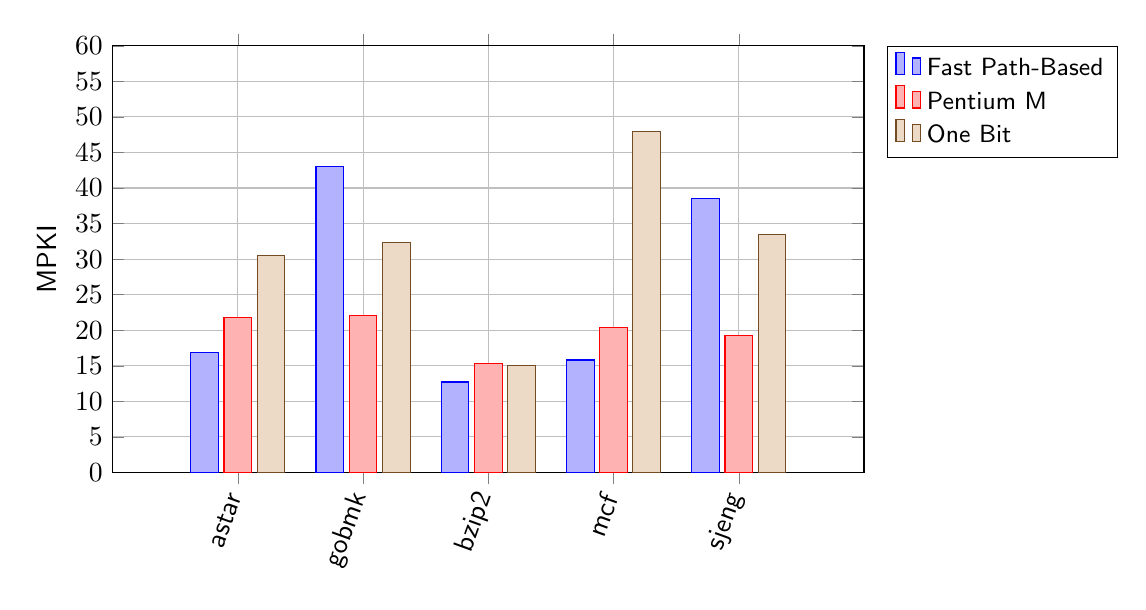
\begin{tikzpicture}
	\begin{axis}[
		width=\textwidth-1cm,
		height=7cm,
		xmin=0, xmax=6,
		ymin=0, ymax=60,
		ylabel=\textsf{MPKI},
		ybar,
		xtick={1,2,3,4,5}, 
		xticklabels={\textsf{astar}, \textsf{gobmk}, \textsf{bzip2}, \textsf{mcf}, \textsf{sjeng}},
		ytick distance ={5},
		xmajorgrids=true,
		ymajorgrids=true,
		x tick label style={rotate=70,anchor=east},
		legend pos=outer north east,
		legend cell align=left,
		legend style={font=\small\sf}
	]
		% own BP
		\addplot
			coordinates {(1,16.84) (2,42.98) (3,12.72) (4,15.81) (5,38.56)};

		% pentium_m
		\addplot
			coordinates {(1,21.79) (2,22.12) (3,15.26) (4,20.43) (5,19.27)};

		% one_bit size 1024
		\addplot
			coordinates {(1,30.45) (2,32.30) (3,15.04) (4,48.00) (5,33.50)};

		\legend{Fast Path-Based, Pentium M, One Bit}
	\end{axis}
\end{tikzpicture}
\caption{MKPI Plot: FPBP compared to Sniper's\cite{carlson2014aeohmcm} build-in branch predictors}
\end{figure}

\begin{figure}[H]
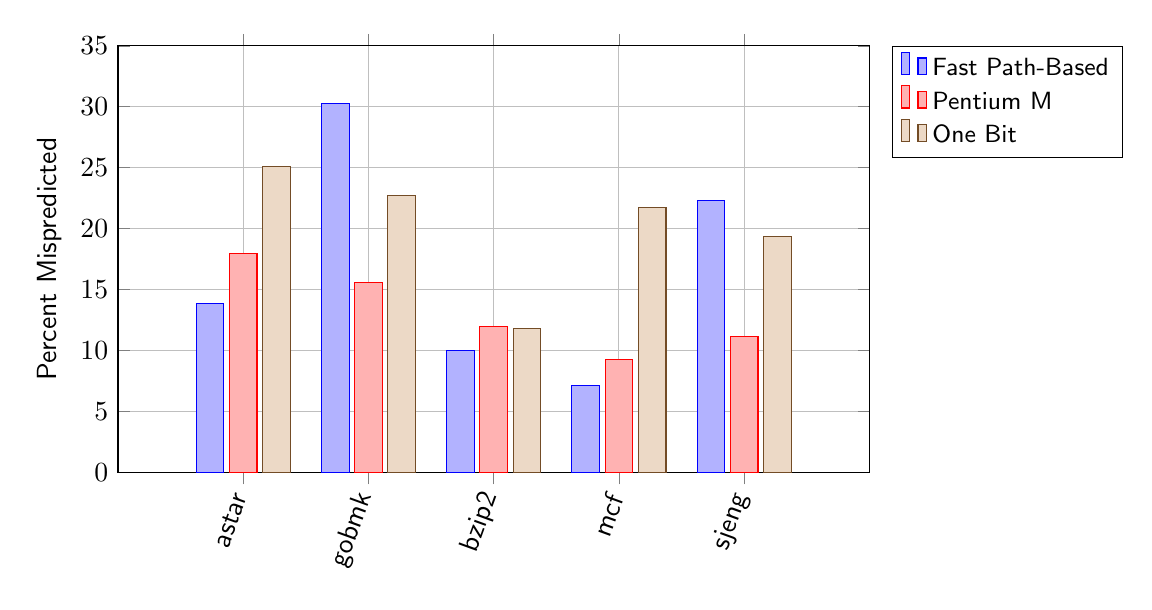
\begin{tikzpicture}
	\begin{axis}[
		width=\textwidth-1cm,
		height=7cm,
		xmin=0, xmax=6,
		ymin=0, ymax=35,
		ylabel=\textsf{Percent Mispredicted},
		ybar,
		xtick={1,2,3,4,5}, 
		xticklabels={\textsf{astar}, \textsf{gobmk}, \textsf{bzip2}, \textsf{mcf}, \textsf{sjeng}},
		ytick distance ={5},
		xmajorgrids=true,
		ymajorgrids=true,
		x tick label style={rotate=70,anchor=east},
		legend pos=outer north east,
		legend cell align=left,
		legend style={font=\small\sf}
	]
		% own BP
		\addplot
			coordinates {(1,13.88) (2,30.25) (3,9.97) (4,7.1) (5,22.29)};

		% pentium_m
		\addplot
			coordinates {(1,17.96) (2,15.57) (3,11.97) (4,9.25) (5,11.14)};

		% one_bit size 1024
		\addplot
			coordinates {(1,25.10) (2,22.73) (3,11.79) (4,21.73) (5,19.37)};

		\legend{Fast Path-Based, Pentium M, One Bit}
	\end{axis}
\end{tikzpicture}
\caption{Mispredicted Percent: FPBP compared to Sniper's\cite{carlson2014aeohmcm} build-in branch predictors}
\end{figure}
Whereas the One Bit branch predictor shows sufficient accuracy for the \textsf{bzip2} benchmark, but its accuracy is much worse for the other benchmarks. This drop in accuracy is due to the simple structure of this predictor. It does not have the ability to detect more complex patterns. The FPBP shows a remarkable different behavior than the two other branch predictors. It performs with superior accuracy for \textsf{astar},\textsf{bzip2} and \textsf{mcf}, but appears to have the worst accuracy for \textsf{gobmk} and \textsf{sjeng}. 
The amount of simulated instructions varies by the fact, that the benchmarks have differant complexity and length. So, first idea was, that the FPBP just needs a minimum amount of instructions to warmup, such that weights are initialized properly.
But the result of the \textsf{astar} benchmark refutes this. The benchmark only uses a small amount of approximately $3.9\text{M}$ instructions compared to the other benchmarks. \ref{tab:instructions}

\begin{table}[H]
	\centering
\begin{tabular}{cc}
	\textbf{Benchmark} & \textbf{Simulated Instructions} \\
	\hline
	astar &  3.9M\\
	gobmk & 140.7M\\
	bzip2 & B\\
	mcf & 1B\\
	sjeng & 234.4M
\end{tabular}
\caption{simulated instructions for each benchmark}
\label{tab:instructions}
\end{table}

Branch Predictors in general ideally should have negligible warmup behavior. A neural predictor which requires a significant warmup to work properly cannot be flexible to future changes in the program flow. 
Observation of the predictor's weights have showed that they already have reasonable values soon after starting the simulation. 

It appears to be true, that the FPBP also suffers from arbitrarily accuracy drops.
The fact that the underlaying structure of this FPBP is similar to a tiny neural network, makes it difficult to understand its final decision-making process. During testing and adjusting the parameters, $hashlen$, the amount of entries related to branch addresses seemed to have a larger impact on accuracy than the history length $h$. This might lead to think, that branch addresses reveal slightly more information about an upcoming branch decision, than the branching history over the last $h$ branches. Given a scenario, with one or more nested loop with large counters and several branches with pseudo random branching behavior inside of the loops, a branch address-oriented predictor definitely performs with better accuracy. Since today's programs indeed can consist of large loops, this scenario might be realistic and give a good explanation of the observed behavior. 
Fully optimizing the parameters remains a NP-hard multivariable problem. Therefore, the author uses this FPBP on top of a simple bimodal branch predictor. How the two branch predictors are combined is not revealed in the paper, but the combination of the two produces remarkable results.
E.g. the \textsf{mcf} benchmark scores for a misprediction rate lower $2\si{\percent}$. Branches of the \textsf{bzip2} can be predicted with an accuracy of larger than $90\si{\percent}$.
The tradeoff of a combined branch predictor is still the hardware overhead of two units with almost the same in functionality and an additional control circuit to combine them.

\section{Verification}
The implementation of the FPBP does not perform as well as promised in the paper. The accuracy is significantly lower than the authors implementation showed in his benchmarks. This might lead to think that the implementation is simply wrong or consists of some tiny mistakes. 
In earlier stages, before debugging, my implementation indeed consisted of a few mistakes. For example, first the branch prediction history and weights were misaligned by one position. Errors like these result in a branch prediction accuracy not significantly better than a random guess. This, and the fact that the neural predictor indeed performs with very high accuracy for some parts during a running application, whereas it does not for other parts, should reduce the chance that the accuracy still suffers from bad mistakes to a negligible amount. Furthermore, the FPBP was able to beat the two default branch predictors One Bit and Pentium M in some benchmarks
\bibliography{references}
\bibliographystyle{unsrt}
\end{document}
